\documentclass[12pt]{article}
\usepackage{latexsym,amsmath,amssymb,tabu,CJKutf8,bm,graphicx}
\usepackage{caption,float}
\usepackage{multirow,booktabs,diagbox}
\textwidth 6.5in \textheight 9in \oddsidemargin 0pt \topmargin -8pt
\pagestyle{plain}

\begin{document}
\begin{CJK}{UTF8}{gkai}	
\title{}
\date{\today}
\author{王鑫}
\maketitle

这里我主要总结了虚单元与谱方法两种方法算出的结果。\\
\section{初值}
 首先两种方法中我给出了相同的初值:\\
 
 $ \mu_+=0 $\\
 
 $ \mu_-=\cos^{2}x+\cos^2 (\frac{x}{2}+\frac{\sqrt{3}y}{2})+\cos^2(-\frac{x}{2}+\frac{\sqrt{3}y}{2})+\cos^{2}(-x)+\cos^2 (-\frac{x}{2}-\frac{\sqrt{3}y}{2})+\cos^2 (\frac{x}{2}-\frac{\sqrt{3}y}{2})$\\
 
 $\mu_-$的图像如下:\\
 \begin{figure}[H]
 	% 调整字体和图片间距;
 	\setlength{\abovecaptionskip}{0.cm}
 	\setlength{\belowcaptionskip}{-0.cm}
 	% 插入子图;
 	\begin{minipage}[!htbp]{0.3\linewidth}
 		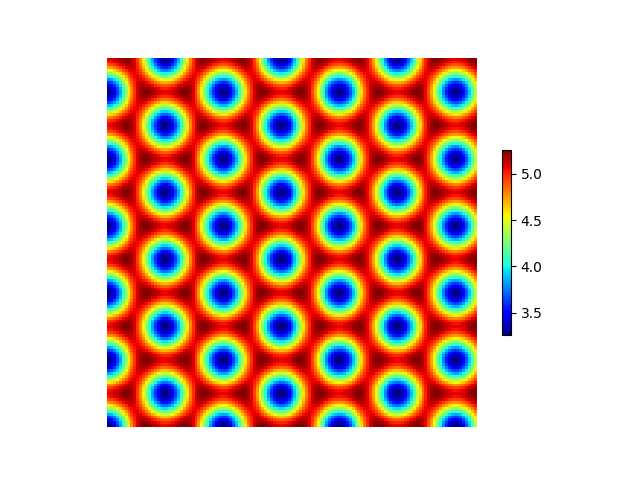
\includegraphics[width=6cm]{Figure_1.png}
 		\caption*{虚单元初值}
 	\end{minipage}
 	\hspace{0.23in}
 	\begin{minipage}[!htbp]{0.3\linewidth}
 		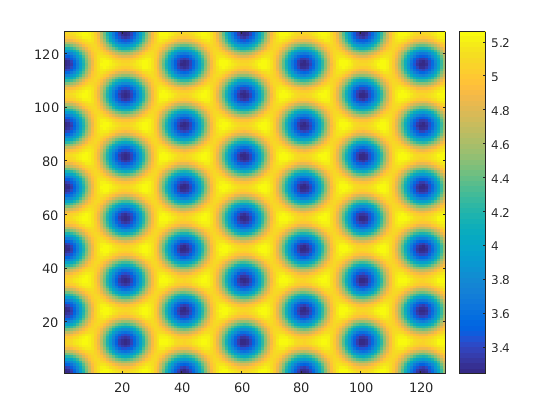
\includegraphics[width=5.2cm]{0.png}
 		\caption*{谱方法初值}
 	\end{minipage}
 \end{figure} 
\section{密度函数$\phi_A$}
下面给出计算过程中重要几步的密度函数$\phi_A$值的图像:\\ 
 \begin{figure}[H]
	% 调整字体和图片间距;
	\setlength{\abovecaptionskip}{0.cm}
	\setlength{\belowcaptionskip}{-0.cm}
	% 插入子图;
	\begin{minipage}[!htbp]{0.3\linewidth}
		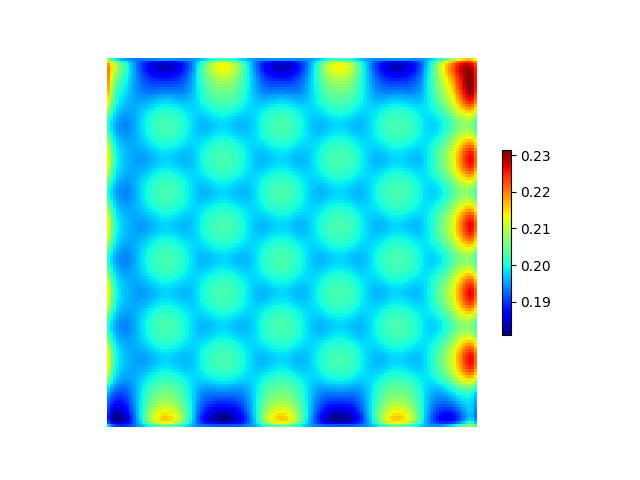
\includegraphics[width=6cm]{scftfigure1.png}
		\caption*{虚单元第一次计算结果}
	\end{minipage}
	\hspace{0.23in}
	\begin{minipage}[!htbp]{0.3\linewidth}
		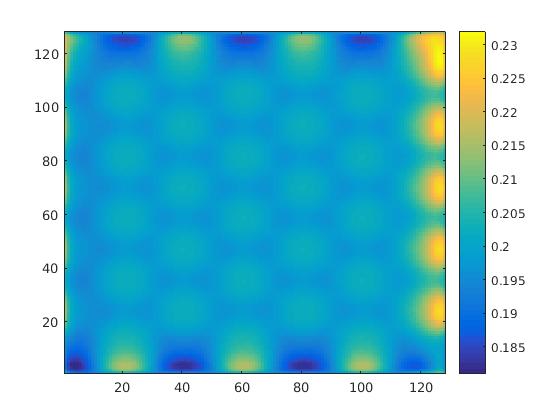
\includegraphics[width=5.2cm]{1.png}
		\caption*{谱方法第一次计算结果}
	\end{minipage}
\end{figure}
  \begin{figure}[H]
 	% 调整字体和图片间距;
 	\setlength{\abovecaptionskip}{0.cm}
 	\setlength{\belowcaptionskip}{-0.cm}
 	% 插入子图;
 	\begin{minipage}[!htbp]{0.3\linewidth}
 		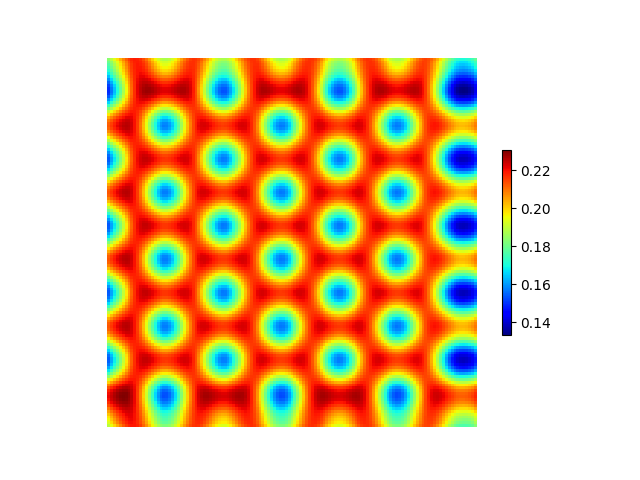
\includegraphics[width=6cm]{scftfigure2.png}
 		\caption*{虚单元第二次计算结果}
 	\end{minipage}
 	\hspace{0.23in}
 	\begin{minipage}[!htbp]{0.3\linewidth}
 		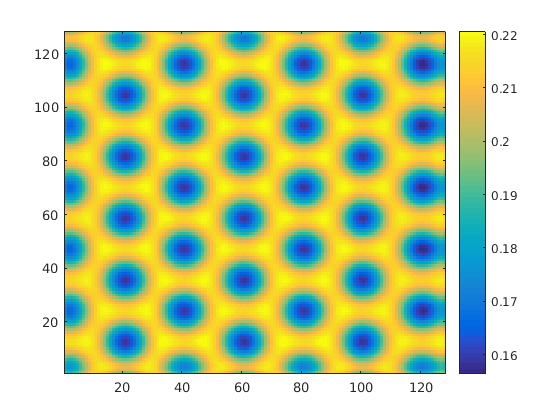
\includegraphics[width=5.2cm]{2.png}
 		\caption*{谱方法第二次计算结果}
 	\end{minipage}
 \end{figure}
  \begin{figure}[H]
	% 调整字体和图片间距;
	\setlength{\abovecaptionskip}{0.cm}
	\setlength{\belowcaptionskip}{-0.cm}
	% 插入子图;
	\begin{minipage}[!htbp]{0.3\linewidth}
		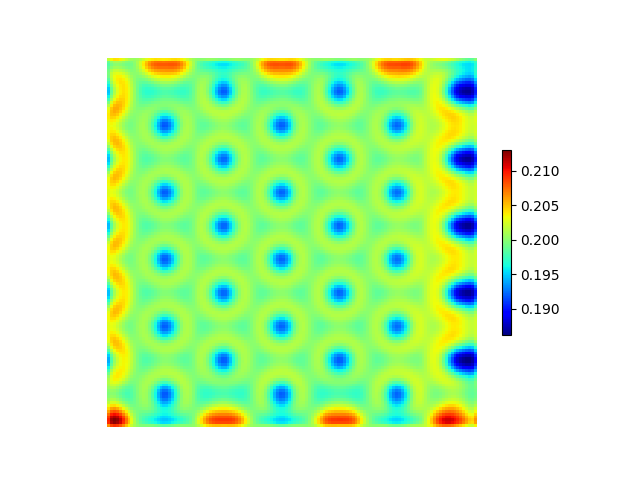
\includegraphics[width=6cm]{scftfigure3.png}
		\caption*{虚单元第三次计算结果}
	\end{minipage}
	\hspace{0.23in}
	\begin{minipage}[!htbp]{0.3\linewidth}
		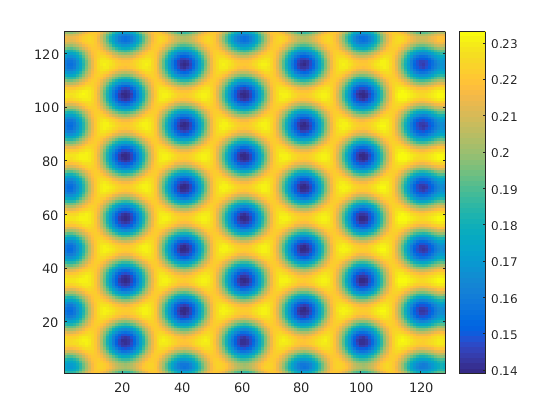
\includegraphics[width=5.2cm]{3.png}
		\caption*{谱方法第三次计算结果}
	\end{minipage}
\end{figure}
  \begin{figure}[H]
	% 调整字体和图片间距;
	\setlength{\abovecaptionskip}{0.cm}
	\setlength{\belowcaptionskip}{-0.cm}
	% 插入子图;
	\begin{minipage}[!htbp]{0.3\linewidth}
		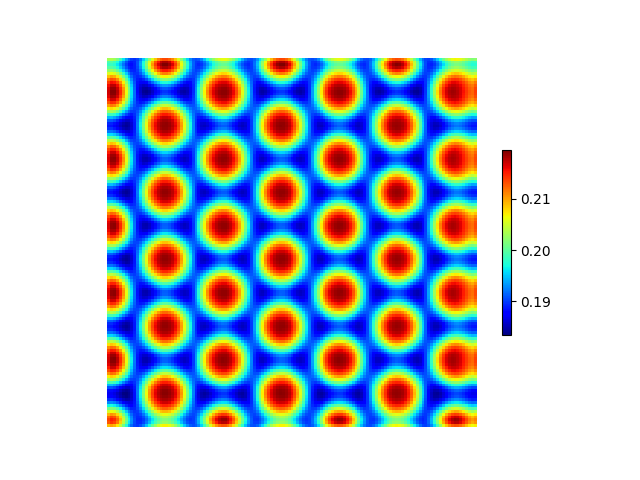
\includegraphics[width=6cm]{scftfigure4.png}
		\caption*{虚单元第四次计算结果}
	\end{minipage}
	\hspace{0.23in}
	\begin{minipage}[!htbp]{0.3\linewidth}
		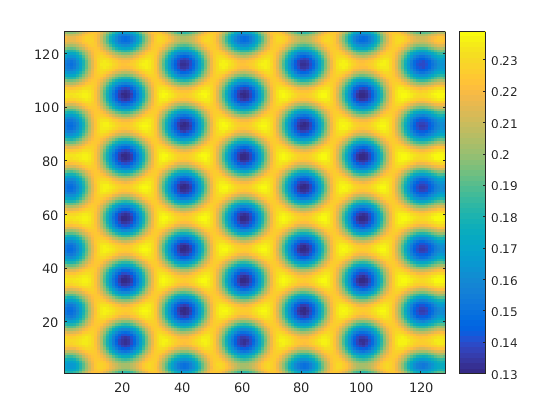
\includegraphics[width=5.2cm]{4.png}
		\caption*{谱方法第四次计算结果}
	\end{minipage}
\end{figure} 
  \begin{figure}[H]
	% 调整字体和图片间距;
	\setlength{\abovecaptionskip}{0.cm}
	\setlength{\belowcaptionskip}{-0.cm}
	% 插入子图;
	\begin{minipage}[!htbp]{0.3\linewidth}
		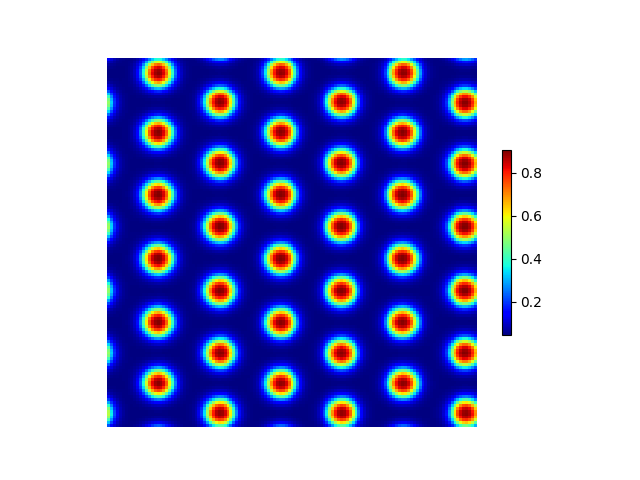
\includegraphics[width=6cm]{scftfigure675.png}
		\caption*{虚单元最终计算结果}
	\end{minipage}
	\hspace{0.23in}
	\begin{minipage}[!htbp]{0.3\linewidth}
		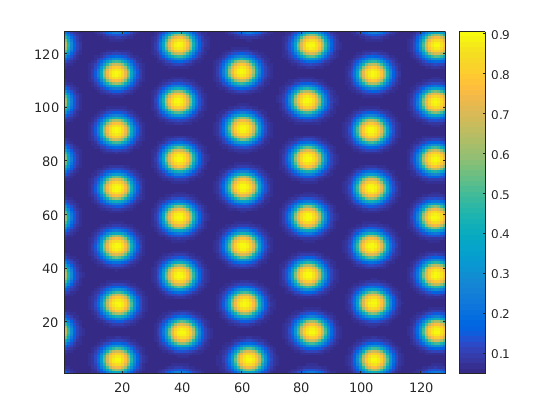
\includegraphics[width=5.2cm]{128.png}
		\caption*{谱方法最终计算结果}
	\end{minipage}
\end{figure}
观察发现第三次的时候两者上下边界已经不同,第四次的时候结果完全不同,最终结果也有区别,但造成这种现象的原因还未发现。

\end{CJK}
\end{document}

